\documentclass[12pt, a4paper]{article}
\usepackage[utf8]{inputenc}
\usepackage{fontenc}
\usepackage{xcolor}
\usepackage{hyperref}
\usepackage[english]{babel}
\usepackage[inline]{enumitem}
\usepackage{graphicx}
\usepackage{cleveref}
\usepackage{enumitem}

\setlist[enumerate,1]{label=\arabic*}
\setlist[enumerate,2]{label=\theenumi.\arabic*}
\setlist[enumerate,3]{label=\theenumii.\arabic*}

\graphicspath{ {res/} }

\newcommand{\versionmajor}{0}
\newcommand{\versionminor}{1}
\newcommand{\versionpatch}{0}
\newcommand{\version}{\versionmajor.\versionminor.\versionpatch}

\title{\LARGE
    Rustfields \\ 
    \small
    Requirements Breakdown Structure
    }

\author{
    Angela Cortecchia \\ 
    \small 
    angela.cortecchia@studio.unibo.it
    \and
    Paolo Penazzi \\ 
    \small
    paolo.penazzi@studio.unibo.it
}

\date{\small }

\begin{document}
\maketitle
\newpage


\section*{Requirements Breakdown Structure}

Il team ha delineato la seguente Requirements Breakdown Structure, riportata di seguito anche con una
rappresentazione grafica.

\subsection*{Goal}

Il goal principale del progetto, individuato dal team è \textbf{estendere ScaFi } una piattaforma che permette
di scrivere programmi aggregati per reti di dispositivi.

\subsection*{Requirements}

A partire dal goal principale del progetto, sono stati individuati diversi requisiti:

\begin{enumerate}
    \item \textbf{Aggregate Computing nativo} Attualmente ScaFi può essere eseguito solo su dispositivi in grado di 
    far girare una JVM. Vogliamo renderlo disponibile anche su dispositivi più leggeri, che non supportano la JVM.
        \begin{enumerate}
            \item \textbf{Esecuzione di un programma aggregato} tutto quello che è necessario per l'esecuzione 
            di un programma aggregato.
            \item \textbf{Scrittura di un programma aggregato} Tutti i costrutti del linguaggio che permettono di 
            scrivere un programma aggregato.
            \item \textbf{Test} L'esecuzione di un programma aggregato deve portare al risultato che ci si aspetta.
        \end{enumerate}

    \item \textbf{Aggiornamento di ScaFi}
        \begin{enumerate}
            \item \textbf{Adottare Scala 3.} Tutto il core attuale è scritto in Scala 2: vogliamo aggiornarlo 
            all'ultima versione di Scala.
            \item \textbf{Espandere la suite di test.} Il core attuale ha una suite di test molto limitata: vogliamo
            espanderla per garantire la correttezza del codice. 
            \item \textbf{Abilitare l'utilizzo di Fields reificati.} Vogliamo abilitare l'utilizzo di Fields reificati
            in ScaFi.
        \end{enumerate}

    \item \textbf{Interoperabilità tra le due versioni:}
        \begin{enumerate}
            \item \textbf{Standardizzare il formato dei messaggi.} La rete che esegue il programma aggregato è composta 
            da dispositivi eterogeneei. Dispositivi di diversi tipi devono poter comunicare tra loro.
            \item \textbf{Implementare un wrapper per il core in Rust.} Un programma aggregato scritto in Scala deve 
            poter essere eseguito da una VM nativa.
        \end{enumerate}
\end{enumerate}

\begin{figure}[h]
    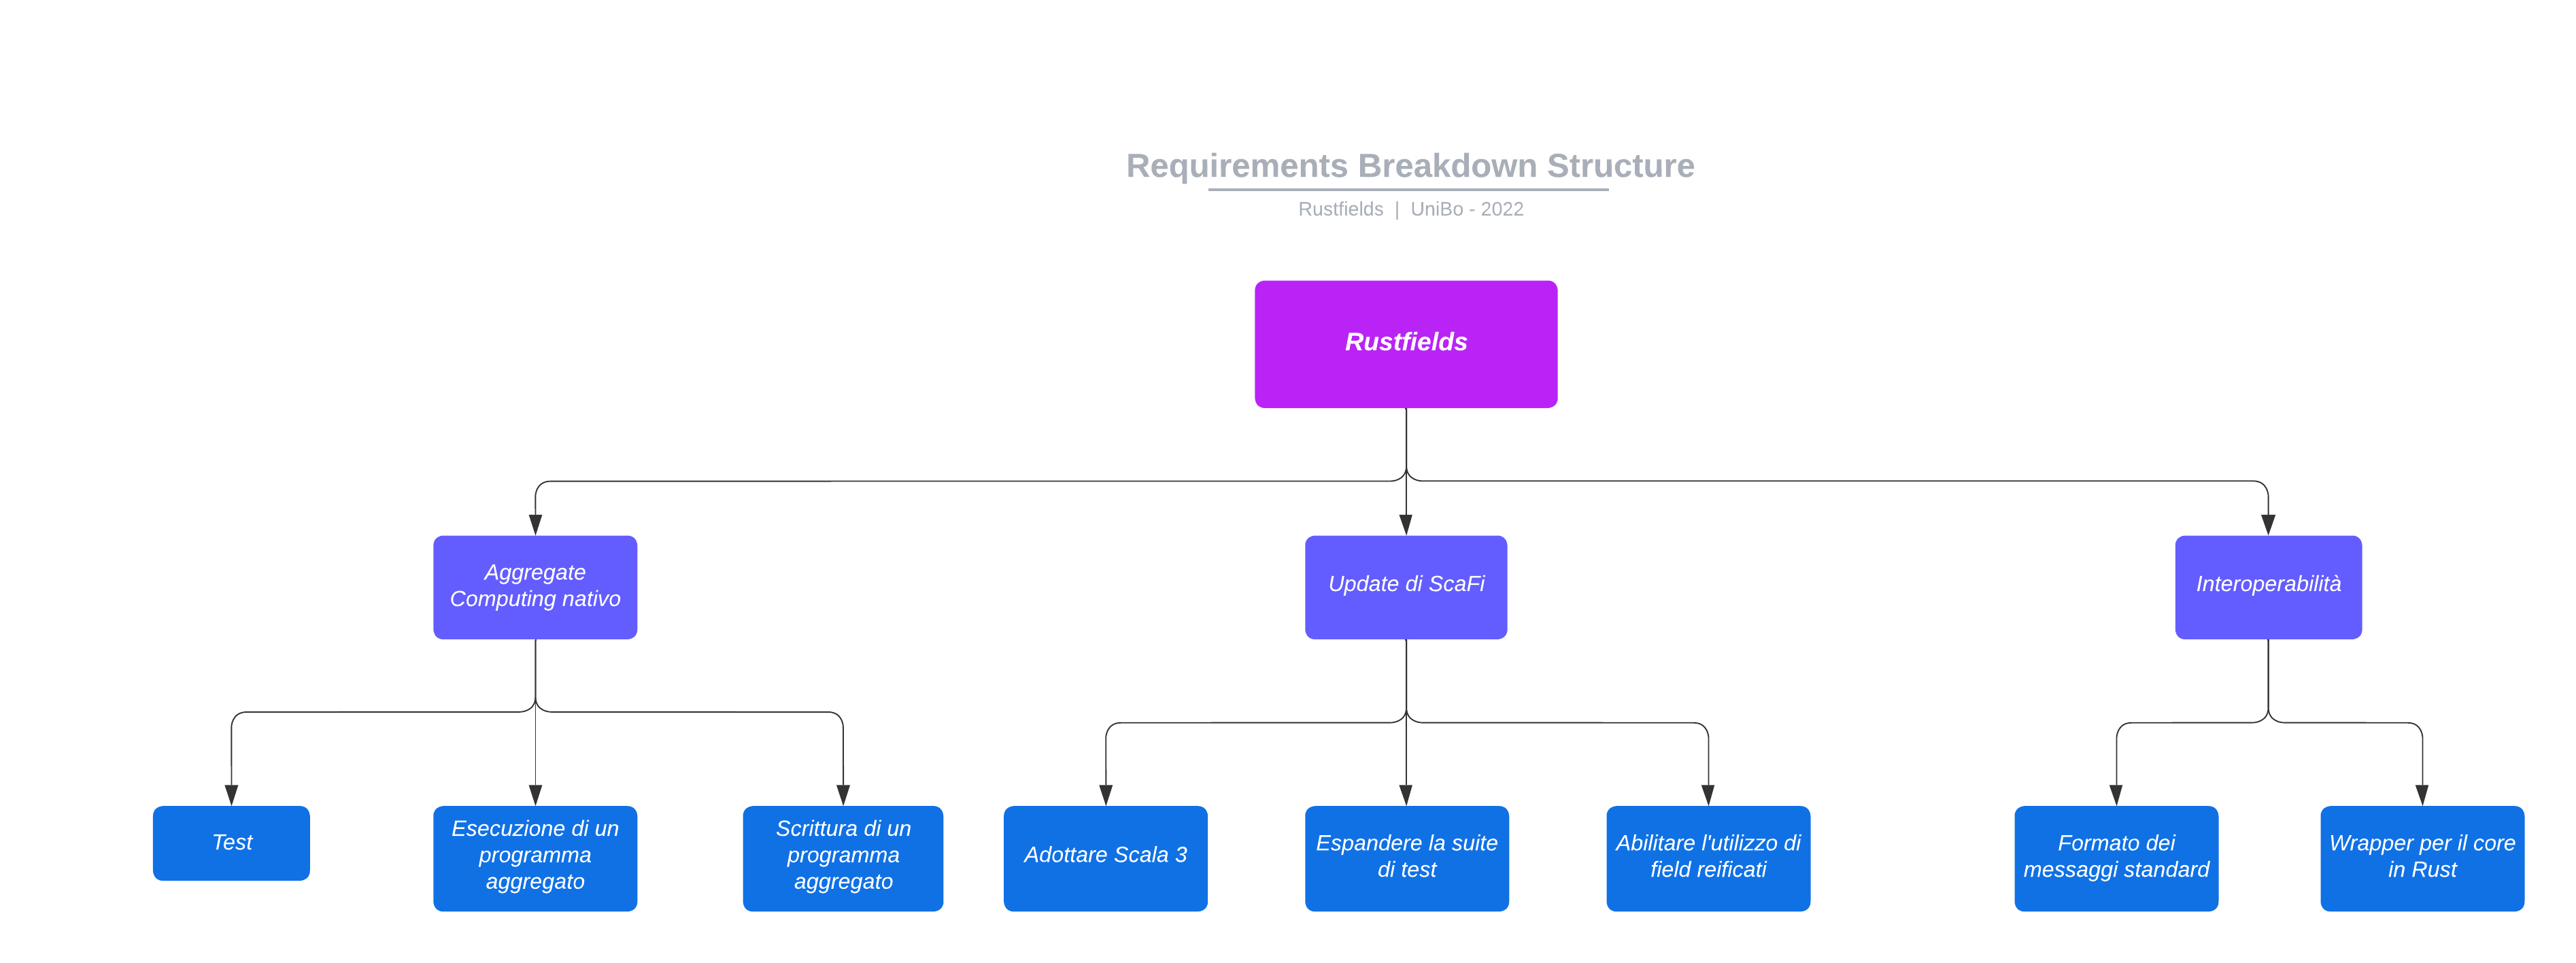
\includegraphics[angle=90, width=\textwidth, height=\textheight]{res/rbs.png}
\end{figure}

\end{document}